\chapter{Grundlagen und Verwandte Arbeiten}

Dieses Kapitel befasst sich mit den technischen Grundlagen dieser Arbeit und verwandten Arbeiten.
Unter den technischen Grundlagen werden zunächst Rahmenwerke erklärt, die im Laufe dieser Arbeit eingesetzt werden.
% ab hier eventuell nochmal bearbeiten
Danach folgt eine genauere Erklärung von Data Lakes.
Zum Schluss wird auf das Change-Data-Capture, zum Erkennen von Änderungen in Daten, eingegangen.

\section{Technische Grundlagen}
\subsection{Hadoop}

Hadoop\footnote{https://hadoop.apache.org/} ist ein Projekt von Apache für die verteilte Datenverarbeitung auf einem Cluster.
Die Verarbeitung basiert auf  Map-Reduce \parencite{mapred}, einem Programmier-Modell, bei dem Daten in Form von Schlüssel-Wert-Paaren verarbeitet werden.
Grob beschrieben, besteht es aus zwei Funktionen.
Die erste ist die Map-Funktion, bei der aus Daten eine Zwischensammlung von Schlüssel-Wert-Paaren erzeugt wird.
Danach werden diese nach den Schlüsseln sortiert und die Reduce-Funktion, zum Zusammenfassen der Paare ausgeführt.
Ein Hadoop-Cluster enthält zwei wichtige Komponenten.
YARN \parencite{yarn} wird für das Ressourcen-Management benutzt.
Die zweite Komponente, das HDFS, ist ein verteiltes und fehlertolerantes Dateisystem, welches ursprünglich für Hadoop entwickelt wurde.
Für dieses Projekt ist nur das HDFS relevant und wird deswegen näher erläutert.

Das HDFS wurde entwickelt, um auf Hardware mit geringen Kosten zu laufen und große Datenmengen zu verarbeiten.
Dateien können von einem Gigabyte bis mehrere Terabyte groß sein.
Die Fehlertoleranz wird dabei durch die Möglichkeit der Replikation mit einem beliebigen Faktor gegeben.

Das Dateisystem ist ähnlich zu anderen bekannten Dateisystemen aufgebaut.
Dateien und Ordner können im Namensraum hierarchisch organisiert werden.
Es unterstützt jedoch keine Zugriffsberechtigung oder Hard- und Soft-Links.
Um einfach und effektiv kohärent zu bleiben, werden Dateien nur einmal geschrieben, können aber mehrfach gelesen werden.
Dateien werden zur Speicherung in einzelne Blöcke aufgeteilt.
Dabei sind für eine Datei alle Blöcke, bis auf den letzten, gleich groß.

\begin{figure}
    \centering
    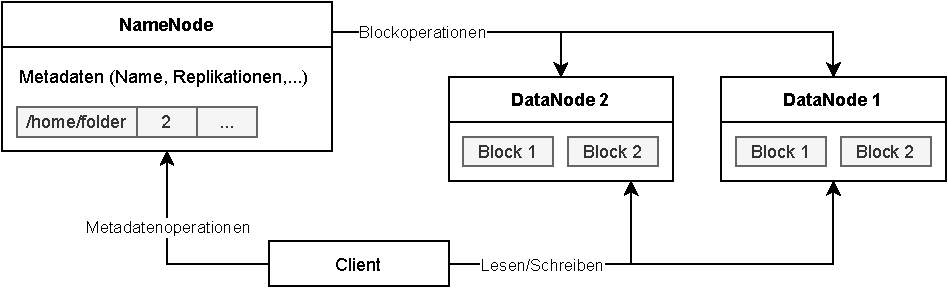
\includegraphics[width=\textwidth]{Grafiken/Grundlagen/HDFS.pdf}
    \caption[HDFS-Architektur]{HDFS-Architektur\footnotemark}
    \label{fig:hdfs-cluster}
\end{figure}
\footnotetext{Nach https://hadoop.apache.org/docs/r1.2.1/images/hdfsarchitecture.gif, Zugriff: 29.12.2021}

Ein HDFS-Cluster (\cref{fig:hdfs-cluster}) funktioniert nach dem Master-Worker-Prinzip und besteht aus einem NameNode und vielen DataNodes.
Der NameNode übernimmt die Verwaltung des Namensraums und die Verteilung der einzelnen Blöcke einer Datei.
Er reguliert dazu noch den Zugriff durch Clients und führt Operationen auf dem Dateisystem, wie das Öffnen, Schließen oder Umbenennen von Ordnern und Dateien aus.
Die DataNodes speichern die einzelnen Blöcke der Dateien.
Auf Anweisung des NameNode werden Blöcke erstellt, gelöscht oder repliziert.
Außerdem bearbeiten sie Anfragen zum Lesen und Schreiben von Dateien \parencite{hdfs}.

% Parquet
Mit Apache Parquet steht ein Format zur Verfügung, mit dem Daten im HDFS effizient gespeichert werden können.
Parquet ist ein spalten-orientiertes Speicherformat, das auch die Kompression und Kodierung der Daten unterstützt.
Über einen Algorithmus zur Zerlegung von Verschachtelung ist auch das Speichern von semistrukturierten Daten möglich \parencite{parquet}.

\subsection{Apache Spark}
\label{sec:spark}

Apache Spark ist eine Datenverabeitungs-Engine für die effiziente, verteilte Verarbeitung von Big Data.
Das Ziel bei der Entwicklung von Apache Spark war es, ein einheitliches Rahmenwerk für Big-Data-Prozesse zu schaffen,
Das Problem war, das die bis dahin verbreitetste Lösung, Hadoop, keine einheitliche Abfragesprache und kein einheitliches Datenmodell hat.
Durch Spark ist das Arbeiten mit zum Beispiel mit SQL, Datenströmen, maschinellem Lernen oder Graph-Daten möglich.
Es gibt viele Bibliotheken für die Verwendung verschiedener Datenquellen in Spark.
Durch ihre Optimierung erreichen diese ähnliche Performance wie manuell dafür implementierte Big-Data-Prozesse.
Spark kann entweder lokal auf einem Computer oder auf einem Spark-Cluster nach dem Master-Worker-Modell ausgeführt werden.

Ein Kernprinzip ist die Abstraktion der Daten in RDDs (Resilient Distributed Datasets, deutsch: Resiliente Verteilte Datensätze).
RDDs sind fehlertolerante Sammlungen von Objekten, die auf die Worker-Instanzen verteilt und parallel bearbeitet werden können.
Diese werden flüchtig im Hauptspeicher gehalten, können aber für spätere schnellere Zugriffe zwischengespeichert (persistiert) werden.
Die Erstellung und Bearbeitung von RDDs geschieht über sogenannte Transformationen.
Die Transformationen werden in einem Herkunftsgraphen gespeichert, wodurch eine Wiederherstellung bei Fehlern an jedem Punkt möglich ist.

Für die Verarbeitung von strukturierten oder semistrukturierten Daten gibt es zusätzlich die eigene Abfragesprache SparkSQL, die sich stark an SQL orientiert.
Es gibt Bibliotheken für die Sprachen Scala, Java, Python und R.
Auf den RDDs gibt es noch eine weitere Abstraktionsebene, die DataFrames.
Mit DataFrames, die eine Sammlung RDDs von Datensätzen mit einem bekannten Schema sind, kann eine API benutzt werden, bei der die Bearbeitung der Daten über Funktionsaufrufe statt SparkSQL möglich ist \parencite{spark}.

Die Interaktion mit einem Spark-Cluster kann über eine interaktive Shell oder eine in einer der unterstützen Sprachen geschriebenen Job geschehen.
Informationen über die Anwendung werden im SparkContext gespeichert.
Beim Lesen und Schreiben wird das Format der Daten angegeben.
Spark unterstützt standardmäßig einige Formate, aber durch die Konfiguration mit zusätzlichen Bibliotheken im SparkContext, kann die Unterstützung weiterer Formate hinzugefügt werden.
Von den verwendeten Bibliotheken und dem Format sind auch die Optionen abhängig, die beim Lesen und Schreiben gesetzt werden müssen.
Die Optionen sind immer Schlüssel-Wert-Paare und enthalten zum Beispiel Verbindungsinformationen zu einer Datenbank oder einen Dateispeicherort \parencite{spark-website}.

\subsection{Apache Kafka}
\label{sec:kafka}

Apache Kafka ist ein verteiltes Event-Streaming-System.
Die Vermittlung der auftretenden Events läuft in Echtzeit ab.
Kafka basiert auf dem nach dem Publish-Subscribe-Modell.
Events können von Produzenten veröffentlicht werden und Konsumenten können auf diese Events abonnieren.
Durch die Verteilung in einem Cluster kann Kafka den Ausfall einzelner Server ausgleichen.
Zusätzlich können Ströme von Events für einen beliebigen Zeitraum gespeichert werden.

Kafka besteht aus einem Cluster von Servern und verschiedenen Clients.
Es gibt zwei Arten von Servern.
Die sogenannten Broaker sind für die Verteilung und Verwaltung von Events zuständig.
Andere verwenden Server Kafka Connect\footnote{https://kafka.apache.org/documentation/\#connect} um existierende Systeme, wie zum Beispiel ein Datenbank-System, in das Kafka-Cluster zu integrieren.
Die Clients sind Anwendungen, die entweder Events produzieren oder konsumieren.

In diesem System repräsentiert ein Event den Fakt, dass etwas "`passiert"' ist und besteht aus einem Schlüssel, einem Wert, einem Zeitstempel und optionalen Metadaten.
Dabei werden die Werte nicht interpretiert sonder einfach als Byte-Block versendet und können so beliebige Struktur haben.
Events werden in sogenannte Topics unterteilt.
Es kann immer mehrere Produzenten oder Konsumenten auf einem Topic geben.
Events in einem Topic können mehrfach gelesen werden und werden nicht nach dem Konsumieren gelöscht.
Es kann aber für jedes Topic eine Dauer festgelegt werden, nach der die Events verworfen werden.
Um ein Topic fehlertolerant zu machen, kann dieses repliziert werden.

Topics werden in Partitionen über verschiedene Broker aufgeteilt, so dass das ganze System gut skalierbar wird.
Ein Produzenten kann zum Beispiel Events auf mehreren Brokern gleichzeitig veröffentlichen.
Wenn ein Event in einem Topic veröffentlicht wird, wird dieses an eine der Partitionen angehängt.
Events, die den gleichen Schlüssel haben werden immer der gleichen Partition zugeordnet und Events einer Partition kommen garantiert in der Reihenfolge des Schreibens bei dem Konsumenten der Partition an \parencite{kafka-docs}.

Konsumenten können auch in Gruppen zusammengefasst werden.
Innerhalb einer Gruppe werden Events eines Topics innerhalb der Mitglieder, die dieses Topic abonniert haben, aufgeteilt.
Diese Funktion kann zum Beispiel für den Lastausgleich verwendet werden.
\pagebreak
\section{Data Lake}
In der Einleitung (\cref{sec:einleitung-datalake}) wurde der Data Lake als Lösung für die Probleme im Big-Data-Bereich bereits kurz beschrieben. 
In diesem Abschnitt wird noch einmal genauer auf Data-Lake-Systeme, deren Definition, Architektur und existierende Systeme eingegangen.

\subsection{Defintion eines Data Lakes}
Neben der, die in der Einleitung gegeben wird, wurde von \textcite{sawadogo2021data} eine detailliertere Definition für Data Lakes aufgestellt.
Hiernach sind Data-Lake-Systeme ein skalierbarer Speicher für Daten jeden Typs.
Die Daten werden im Rohformat gespeichert und hauptsächlich durch Datenspezialisten, wie Statistiker oder Analysten, für die Extraktion von Wissen verwendet.
Ein Data Lake hat dabei die folgenden Eigenschaften: \begin{enumerate}
    \item ein Metadaten-Katalog, um die Datenqualität sicher zu stellen,
    \item Regeln und Werkzeuge für die Data Governance,
    \item Zugänglichkeit zu den Daten für verschiedene Arten von Benutzern,
    \item die Integration von Daten jeden Typs,
    \item sowohl eine logische als auch eine physische Gliederung und
    \item die Skalierbarkeit von Speicher und Verarbeitung.
\end{enumerate}

\subsection{Architekturen für Data Lakes}
Von \textcite{inmon2016data} wird das System in sogenannten Ponds (Teiche) strukturiert.
Jeder Pond ist mit einem spezialisierten Speichersystem verknüpft und beinhaltet Daten eines bestimmten Typs.
Einige Ponds führen zudem weitere Verarbeitungen der Daten, wie Aufbereitung oder Analysen aus.
Inmon hat eine Architektur aus fünf Ponds aufgestellt (\cref{fig:datalake-ponds}).
\begin{enumerate}
    \item Daten werden im Raw Data Pond im Rohformat gespeichert und fließen von dort aus in andere Teiche.
    Dieser dient also als Eintrittspunkt in das System für neue Daten.
    Nach dem Verlassen des Teichs werden die aus diesem Daten gelöscht.
    \item Der Analog Data Pond enthält analoge Daten, meist von IoT-Geräten.
    Diese werden hier auf ein aussagekräftiges und verwaltbares Volumen reduziert und umstrukturiert.
    \item In den Application Data Pond kommen Daten, die von Software-Anwendungen erzeugt wurden.
    Diese sind häufig strukturierte Daten aus relationalen Datenbank-Systemen.
    Sie werden für Analysen integriert und aufbereitet.
    \item Der Textual Data Pond enthält unstrukturierte Daten und Prozesse, die deren Analyse erleichtern.
    \item Im Archival Data Pond werden alle Daten gespeichert, die nicht mehr aktiv verwendet, aber eventuell in der Zukunft nochmal gebraucht werden.
\end{enumerate}
\begin{figure}
    \centering
    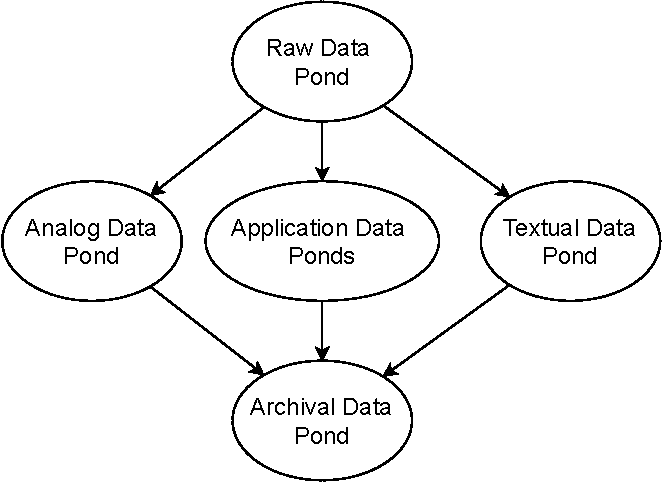
\includegraphics[width=.8\textwidth]{Grafiken/Grundlagen-Ponds.pdf}
    \caption{Ponds-Architektur eine Data Lakes nach Inmon}
    \label{fig:datalake-ponds}
\end{figure}

Ein anderer Ansatz ist die Unterteilung des Data Lakes in Zonen (\cref{fig:datalake-zones}).
Hier werden die Daten nach ihrem Verfeinerungsgrad in einer entsprechenden Zone abgelegt.
Dabei durchlaufen sie die einzelnen Zonen hintereinander.
Die Anzahl der Zonen und deren Verfeinerungsgrad ist dabei je nach Anwendung unterschiedlich \parencite{dl-zones}.

\begin{figure}
    \centering
    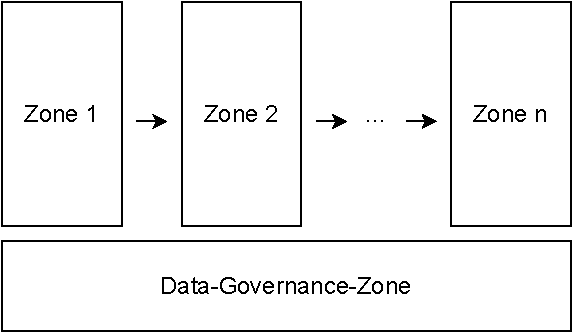
\includegraphics[width=.8\textwidth]{Grafiken/Grundlagen-Zones.pdf}
    \caption{Prinzip der Zonen-Architektur}
    \label{fig:datalake-zones}
\end{figure}

Eine speziellere Architektur ist die Lambda-Architektur, die für die verteilte Verarbeitung von Echtzeit- und Batch-Daten verwendet wird.
Eine Lambda-Architektur besteht aus drei Ebenen (Layers) \parencite{lambda-arch}. \begin{enumerate}
    \item Die Batch Layer hat zwei Aufgaben.
    Die erste Aufgabe ist das verteilte Speichern von wachsenden Daten.
    Dafür kann zum Beispiel das HDFS verwendet werden.
    Als zweite Aufgabe werden Batch Views für die verteilten Daten vorberechnet, um Anfragen schneller beantworten zu können.
    \item In der Speed Layer werden inkrementell Echtzeit-Views auf Daten verwaltet.
    Dadurch wird die Lücke gefüllt, die bei den Views in der Batch-Ebene entstehen können.
    Die Speed Layer enthält immer nur aktuelle Daten.
    Ältere Daten werden durch die Batch Layer aufgenommen.
    \item Die Serving Layer enthält Indices über alle Batch Views um Anfragen mit geringer Latenz bearbeiten zu können. Sie ist dafür verantwortlich die Views aus der Batch und der Speed Layer zusammenzuführen um Echtzeitergebnisse über alle Daten bereit zu stellen.
\end{enumerate}

Nach \textcite{sawadogo2021data} können die Architekturen von Data-Lake-System anders unterteilt werden.
Bei datenorientierten Architekturen wird der Data Lake in verschiedene Datenbereiche unterteilt.
Die funktionsorientierten Architekturen dagegen teilen das Data-Lake-System nach den Funktionen auf, die in ähnlichen Bereichen zusammengefasst werden.
Ein Beispiel ist die Architektur aus der Einleitung von \textcite{datalake_03}.
In hybriden Architekturen können auch beide Ansätze kombiniert werden.

\subsection{Existierende Data-Lake-Systeme und Rahmenwerke}
Es gibt bereits verschiedene Rahmenwerke oder Systeme für die Umsetzung eines Data Lakes.
Nachfolgend wird eine Auswahl daraus vorgestellt.

\paragraph{CoreDB} CoreDB ist ein Service, der es erlaubt über eine einzige REST-API Daten und Metadaten in einem Data Lake zu organisieren, zu indizieren und ab zu fragen. 
Es können sowohl relationale als NoSQL-Datenbanksysteme mit CoreDB verwendet werden.
Für die Suche in den Daten wird elastic\footnote{https://www.elastic.co/} verwendet.
Das Design von CoreDB unterstützt sowohl Sicherheit und Zugriffskontrolle als auch Verfolgung und Herkunft um überwachende Metadaten sammeln zu können \parencite{coredb}.

\paragraph{Azure Data Lake} In dem Cloud-Angebot von Microsoft gibt es den Azure Data Lake\footnote{https://azure.microsoft.com/de-de/solutions/data-lake/}.
Hier werden viele Funktionen, die für den Aufbau eines Data Lakes notwendig sind als Cloud-Lösung bereitgestellt.
Dazu gehören unter anderem Hadoop, Apache Spark und ein Speichersystem zum Speichern aller Daten.
Außerdem gibt es weitere Dienste zur Analyse oder Integration der Daten.

\paragraph{Kylo} Kylo\footnote{https://kylo.io/} ist ein Projekt für eine Data-Lake-Management-Plattform.
In dieser Plattform ist eine Ingestion-Komponente enthalten, die die Bereinigung und Validierung von Daten unterstützt.
Außerdem gibt es Funktionen für die Aufbereitung und Erkundung von Daten oder zur Systemüberwachung.
Zusätzlich ist Apach Nifi\footnote{https://nifi.apache.org/} zur Erstellung von Verarbeitungs-Pipelines integriert.
Die Entwicklung an Kylo wird seit über einem Jahr nicht mehr fortgeführt.

\paragraph{Hudi} Apache Hudi\footnote{https://hudi.apache.org/} ist eine Plattform, um selbst-verwaltete Data Lakes mit einer Optimierung für Datenstromverarbeitung aufzubauen.
Zu den Features von Hudi gehört zum Beispiel die Indizierung von Änderung und das Zurückgehen in den Daten zu einem bestimmten Zeitpunkt.
Hudi unterstützt sowohl inkrementelle Abfragen als auch Batch-Verarbeitung von Daten.

\paragraph{}
Bei diesen System fehlen entweder eine ausführliche Metadatenpflege oder eine Daten Versionierung, sie bilden nur einen bestimmten Teil eines Data Lakes oder sind für spezielle Anwendungsfälle.
Daher wurde bisher kein geeignetes Data-Lake-System für die Anwendung am HIT gefunden.

\subsection{Delta Lake}

Als eine Lösung für die Versionierung von Daten gibt es den Delta Lake
Delta Lake ist eine extra Speicherebene, die auf dem HDFS oder eine Objektspeicher in der Cloud, wie Amazons S3, angewendet werden kann.
Das Ziel ist es, diesen Speichern ACID-Transaktionen, schnelles Arbeiten mit Metadaten der Tabelle und eine Versionierung der Daten hinzuzufügen.
Daten werden in sogenannten Delta-Tabellen mit Metadaten und Logs gespeichert.

Eine Delta-Tabelle wird zunächst durch ein Verzeichnis im Dateisystem dargestellt.
Die tatsächlichen Daten werden in diesem Verzeichnis als Parquet-Dateien abgelegt.
Dabei können die Daten auch noch in Unterverzeichnisse aufgeteilt werden, zum Beispiel für jedes Datum ein Verzeichnis.
Neben den Datenverzeichnissen gibt es in jeder Delta-Tabelle einen Ordner für die Logs in Form von JSON Dateien mit aufsteigender Nummerierung.
Metadaten werden sowohl innerhalb der Parquet- als auch in der Log-Dateien gespeichert.

Im Delta Lake wird ein Protokoll für den Zugriff verwendet, dass es mehreren Clients ermöglicht gleichzeitig Lesen zu können, aber immer nur einem das Schreiben erlaubt.
Dabei werden beim Schreiben immer erst neue Datensätze, die zur Tabelle hinzugefügt werden sollen, in das Verzeichnis der Delta-Tabelle geschrieben.
Danach wird eine neu Log-Datei erstellt.

Beim Lesen werden die Log-Dateien als Grundlage verwendet um daraus zusammen mit den gespeicherten Daten den Zustand der Tabelle an einem bestimmten Zeitpunkt zu erzeugen.
Standardmäßig wird beim Lesen immer die aktuellste Version verwendet, man kann aber auch eine bestimmte Version angeben.
Um den Aufwand bei der Verarbeitung der Logs zu verringern wird periodisch ein Kontrollpunkt erzeugt, bei dem alle vorherigen Logs zusammengefügt und komprimiert werden.
Das bedeutet, dass zum Beispiel das Operationen die sich gegenseitig aufheben nicht gespeichert werden.
Damit reicht es aus nur den letzten Checkpoint vor der zu lesenden Version und alle darauf folgende Logs zu lesen.

Durch das Design werden keine eigenen Server für die Pflege der Delta-Tabellen benötigt.
Diese Funktionen werden von den Clients übernommen.
Der Delta Lake unterstützt sowohl die Batch-Verarbeitung von Daten als auch Datenströme und bietet volle Integration in Spark \parencite{deltalake}.


\subsection{Existierender Data-Lake-Prototyp}
In einem Masterprojekt an der Hochschule Niederrhein \parencite{prototyp} wurde ein Prototyp für ein Data-Lake-System entwickelt.
In \cref{fig:prototyp-architektur} ist ein Überblick über dessen Architektur zu sehen.
Es handelt sich hierbei um eine Client-Server-Anwendung.
Der Client besteht aus einer Web-Anwendung über die Benutzer mit dem Data-Lake-System interagieren.
Er kommuniziert mit dem Server über eine REST-API, die auch durch andere Clients verwendet werden könnte.
Die Datenverarbeitung wird über ein Spark-Cluster gelöst.
Zum Speichern der Daten stehen drei verschiedene System zu Verfügung.
Es kommen eine PostgreSQL Datenbank für strukturierte, eine MongoDB für semistrukturierte und ein HDFS für unstrukturierte Daten zum Einsatz.

\begin{figure}
    \centering
    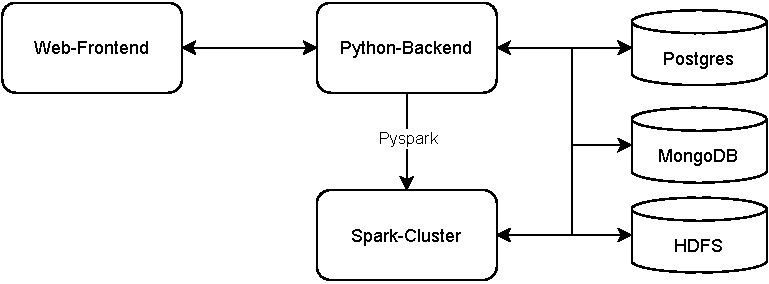
\includegraphics{Grafiken/Prototyp-Architektur.pdf}
    \caption[Architektur des Prototyp]{Architektur des Prototyp}
    \label{fig:prototyp-architektur}
\end{figure}

Die Verarbeitung der Ingestion ist im Prototyp abhängig von der Datenquelle und dem ausgewählten Zielspeicher.
In \cref{fig:prototyp-ingestion}  sind die verschiedenen Wege zu sehen.
Diese Verarbeitungsweise hat zwei Probleme, die in der neuen Ingestion gelöst werden müssen.
Dadurch, dass der Benutzer aus den verschiedenen Speichern ein Ziel auswählt, können hier leicht Probleme entstehen, falls die Datenquelle nicht mit dem Format des Speichers kompatibel ist.
Außerdem sind die Verarbeitungen der Quellen zu den Speichern fest im Code des Servers einprogrammiert.
So ist es nicht möglich während der Laufzeit neue Datenquellen zu integrieren.

\begin{figure}
    \centering
    \subfigure[Datenbank-Ingestion]{
        \label{fig:prototyp-db-ingeston}
        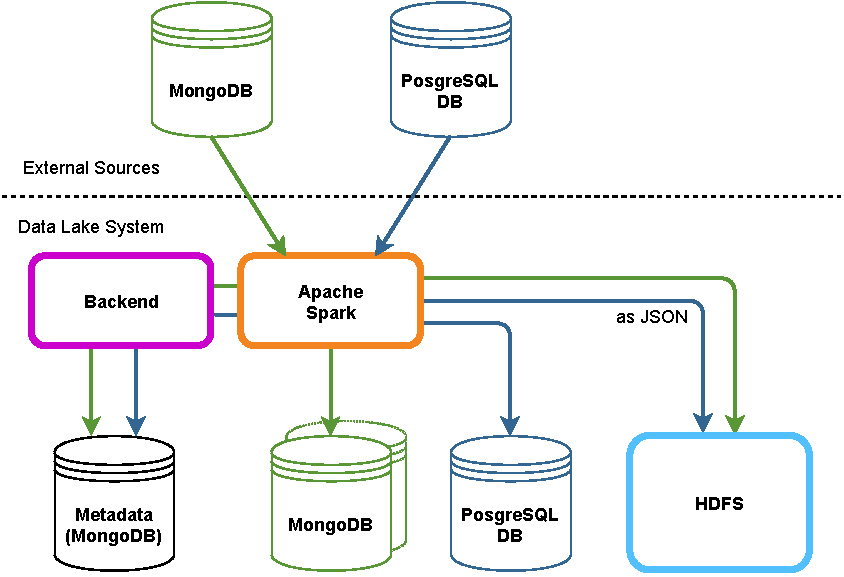
\includegraphics[width=.45\textwidth]{Grafiken/db_ingestion.pdf}
    }
    \subfigure[Datei-Ingestion]{
        \label{fig:prototyp-file-ingeston}
        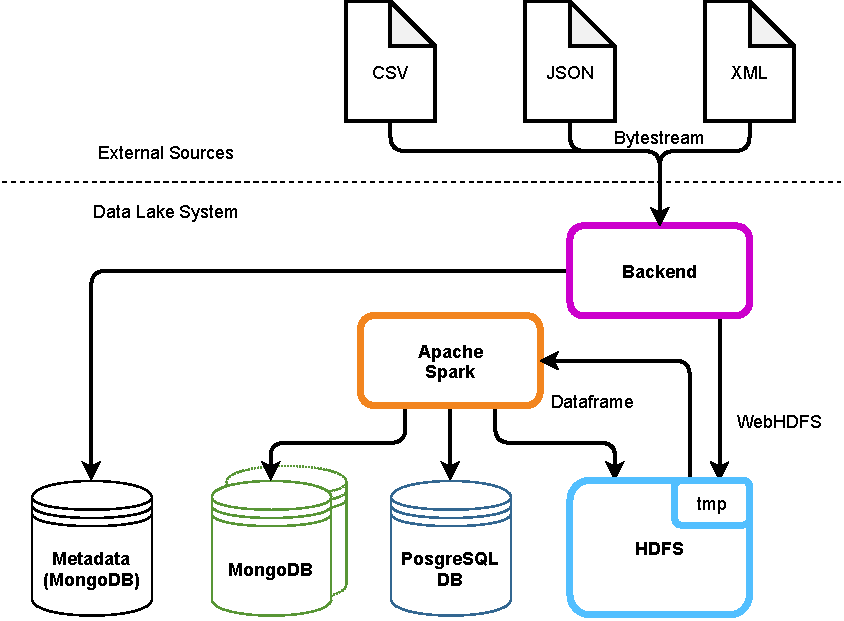
\includegraphics[width=.45\textwidth]{Grafiken/file_ingestion.pdf}
    }
    \caption[Ingestion-Verarbeitung des Prototyp]{Ingestion-Verarbeitung des Prototyp, \textcite[Quelle:][S. 3]{prototyp}}
    \label{fig:prototyp-ingestion}
\end{figure}

Im Vorlauf dieser Arbeit wurde ein Refactoring des Prototyp durchgeführt.
Dabei wurde festgestellt, dass die Erweiterung des Data-Lake-Systems um die Kompatibilität mit weiteren Datenquellen ein aufwändiger Prozess ist.
Auch durch die gewählten Speichersysteme für die geladenen Daten erschweren die Integration einer Lösung für die Versionierung der Daten.
Daher wurde beschlossen, dass eine dedizierte Ingestion-Schnittstelle für das System entwickelt werden soll.

\section{Change Data Capture}
\label{sec:cdc}

Um Änderungen an Daten in Datenquellen in das Data-Lake-System einpflegen zu können, müssen diese erst erfasst werden.
Diesen Prozess nennt man Change-Data-Capture (CDC).
Das Ziel beim CDC ist es, die Änderungen an den Daten nur an einer Stelle zu erfassen und dann an andere Systeme weiter zu geben, damit folgende Verarbeitungsschritte nur die Änderungen berücksichtigen und nicht auf den gesamten Datenbestand zurückgreifen müssen.
Dafür gibt es verschiedene Ansätze, die auf Datenbank-Triggern \parencite{boeing}, Log-Einträgen \parencite{delta-view_gen}, Zeitstempeln \parencite{delta-view_gen, boeing} oder Snapshots \parencite{cdc_in_nosql} basieren.

\subsection{Änderungserfassung Datenbank-Triggern}
Datenbank-Trigger sind Funktionen, die bei verschiedenen Aktionen auf den Daten in einer Datenbank ausgelöst werden.
Über diese Trigger lassen sich CDC-Programme realisieren, die Änderungen genau dann festhalten, wenn sie geschehen.
Ein Nachteil ist, dass die Methode nur in Systemen angewendet werden kann, die auch Trigger unterstützen.
Dafür ist es möglich alle Änderungen wie Einfügen, Aktualisieren oder Löschen von Daten zu erfassen \parencite{boeing}.

\subsection{Log-basierte Änderungserfassung}
Es gibt viele Datenspeicher-Systeme, die Logs über die Aktionen auf den Daten führen.
Diese werden zum Beispiel genutzt, um eine Wiederherstellung möglich zu machen.
Ein CDC-Programm kann diese Logs auslesen und daraus die Änderungsdaten erzeugen.
Hierdurch gibt es fast keinen zusätzlichen Aufwand für das eigentliche System.
Aber auch hier gilt, dass diese Methode davon abhängig ist ob ein System Logs erstellt und ob diese durch externe Programme abgerufen werden können \parencite{delta-view_gen}.


\subsection{Zeitstempel-basierte Änderungserfassung}
Ein weiterer Ansatz ist die Verwendung von Zeitstempeln mit den Zeitpunkten der Erstellung und letzten Änderung.
Diese Zeitstempel müssen in jedem Datensatz vorhanden sein.
Die Verantwortung dafür kann entweder bei dem Ersteller der Daten liegen oder durch das Speichersystem automatisch hinzugefügt werden.
Das CDC-Programm überprüft regelmäßig alle Zeitstempel der Einträge in den Daten.
Wenn diese zwischen dem letzten und dem aktuellen Durchlauf liegen wird die Änderung erfasst.
Hierbei werden nur kumulierte Änderungen seit dem letzten Durchlauf erfasst.
Es ist nicht möglich nachzuvollziehen, welche und wie viele Änderungen in der Zeit gemacht wurden.
Außerdem lassen sich auch mit dieser Methode kein Löschungen erfassen \parencite{delta-view_gen}.
Der Aufwand für diese Methode kann relativ hoch werden, da ohne Indices auf den Zeitstempeln immer die gesamten Daten gelesen werden müssen \parencite{boeing}.

\subsection{Snapshot-basiert Änderungserfassung}
\label{sec:snaps}
Die letzte Methode ist das Vergleichen zweier Momentaufnahmen (Snapshots) eines Datensatzes.
Dabei wird bei jedem Durchlauf zuerst ein aktueller Snapshot generiert.
Dieser wird danach mit dem des vorherigen Durchlaufs verglichen, um alle Änderungen zu erhalten.
Hierfür muss ein separater Speicherort für die Snapshots festgelegt werde.
Wie bei den Zeitstempeln ist es nicht möglich den gesamten Änderungsverlauf zwischen zwei Snapshots nachzuvollziehen.
Außerdem müssen für den Vergleich immer alle Daten geladen werden, was zu einem hohen Rechen- und Speicheraufwand führen kann \parencite{cdc_in_nosql}.